%!TEX root = ../thesis.tex
% appendix section 4

\chapter{Experimental sequences}
\label{sec:ap4}

Below are the experimental sequences used for all diagnostics on laser produced plasma:

\begin{figure}[ht!]
\centering
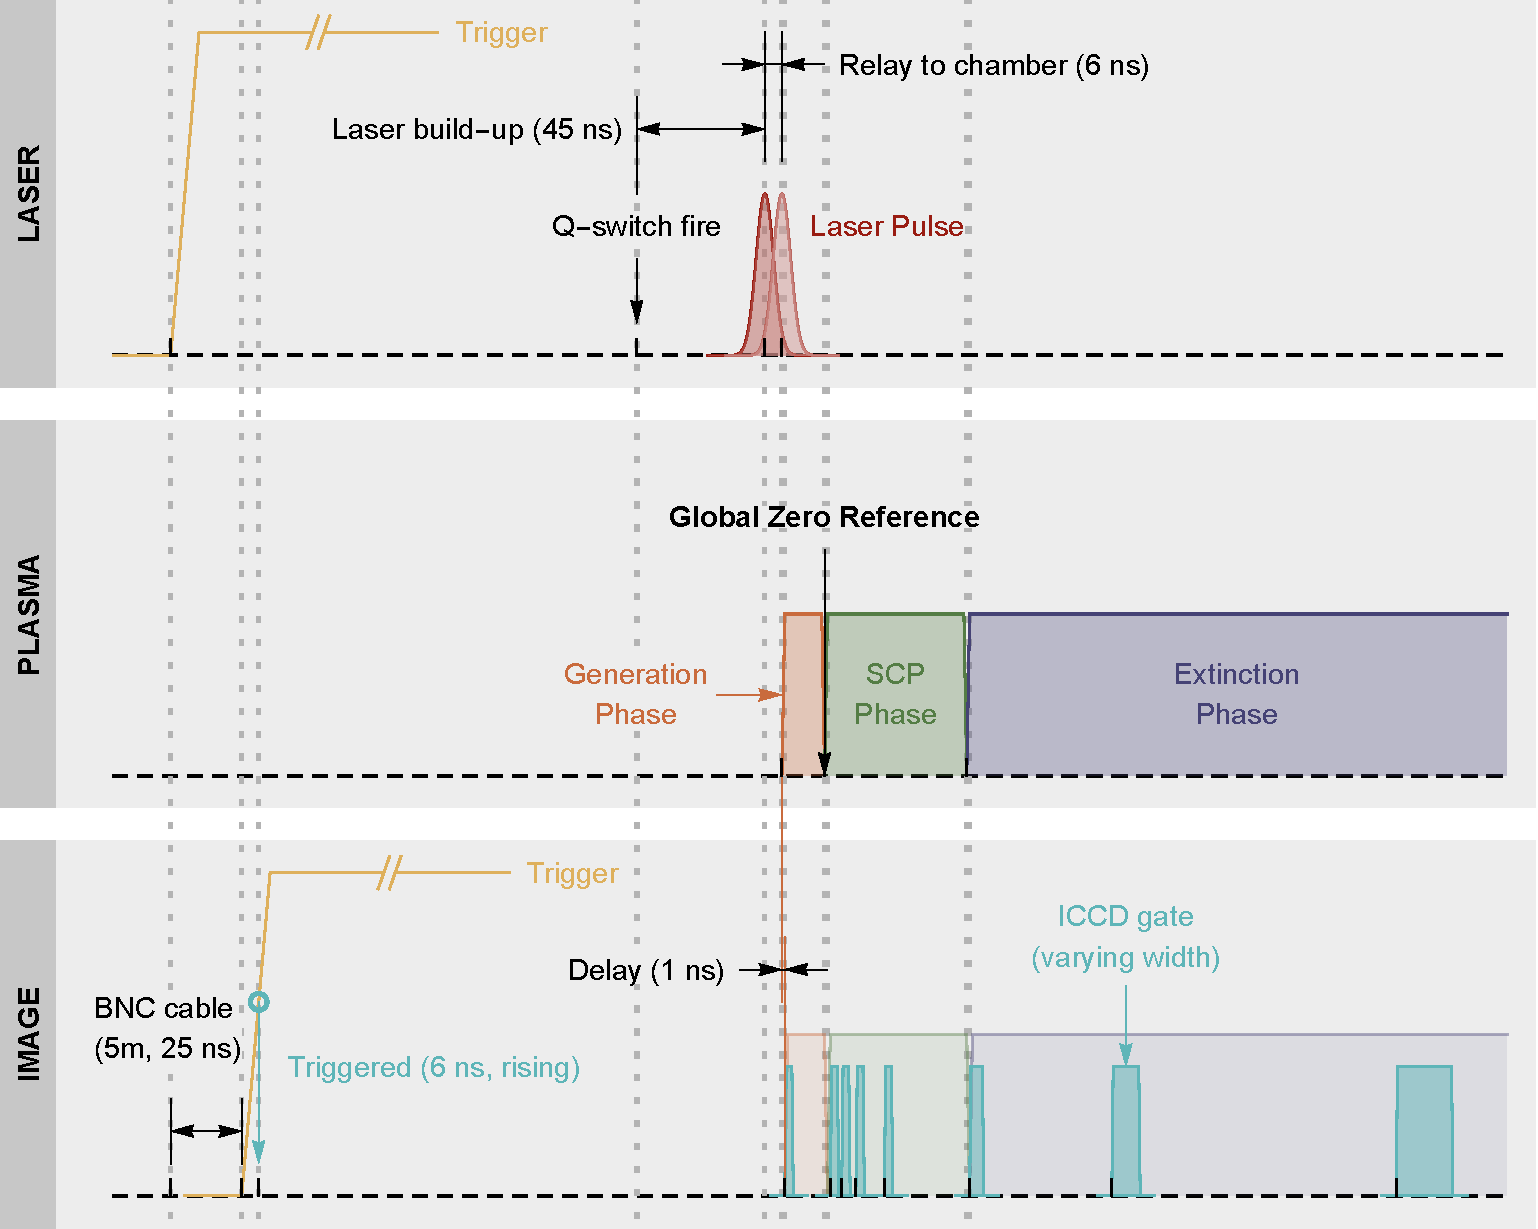
\includegraphics[width=130mm]{figures/ap4/sequence/imgSequence.pdf}
\caption{Experimental sequence for taking images from the plasma.}
\label{fig:imgSequence}
\end{figure}

\begin{figure}[ht!]
\centering
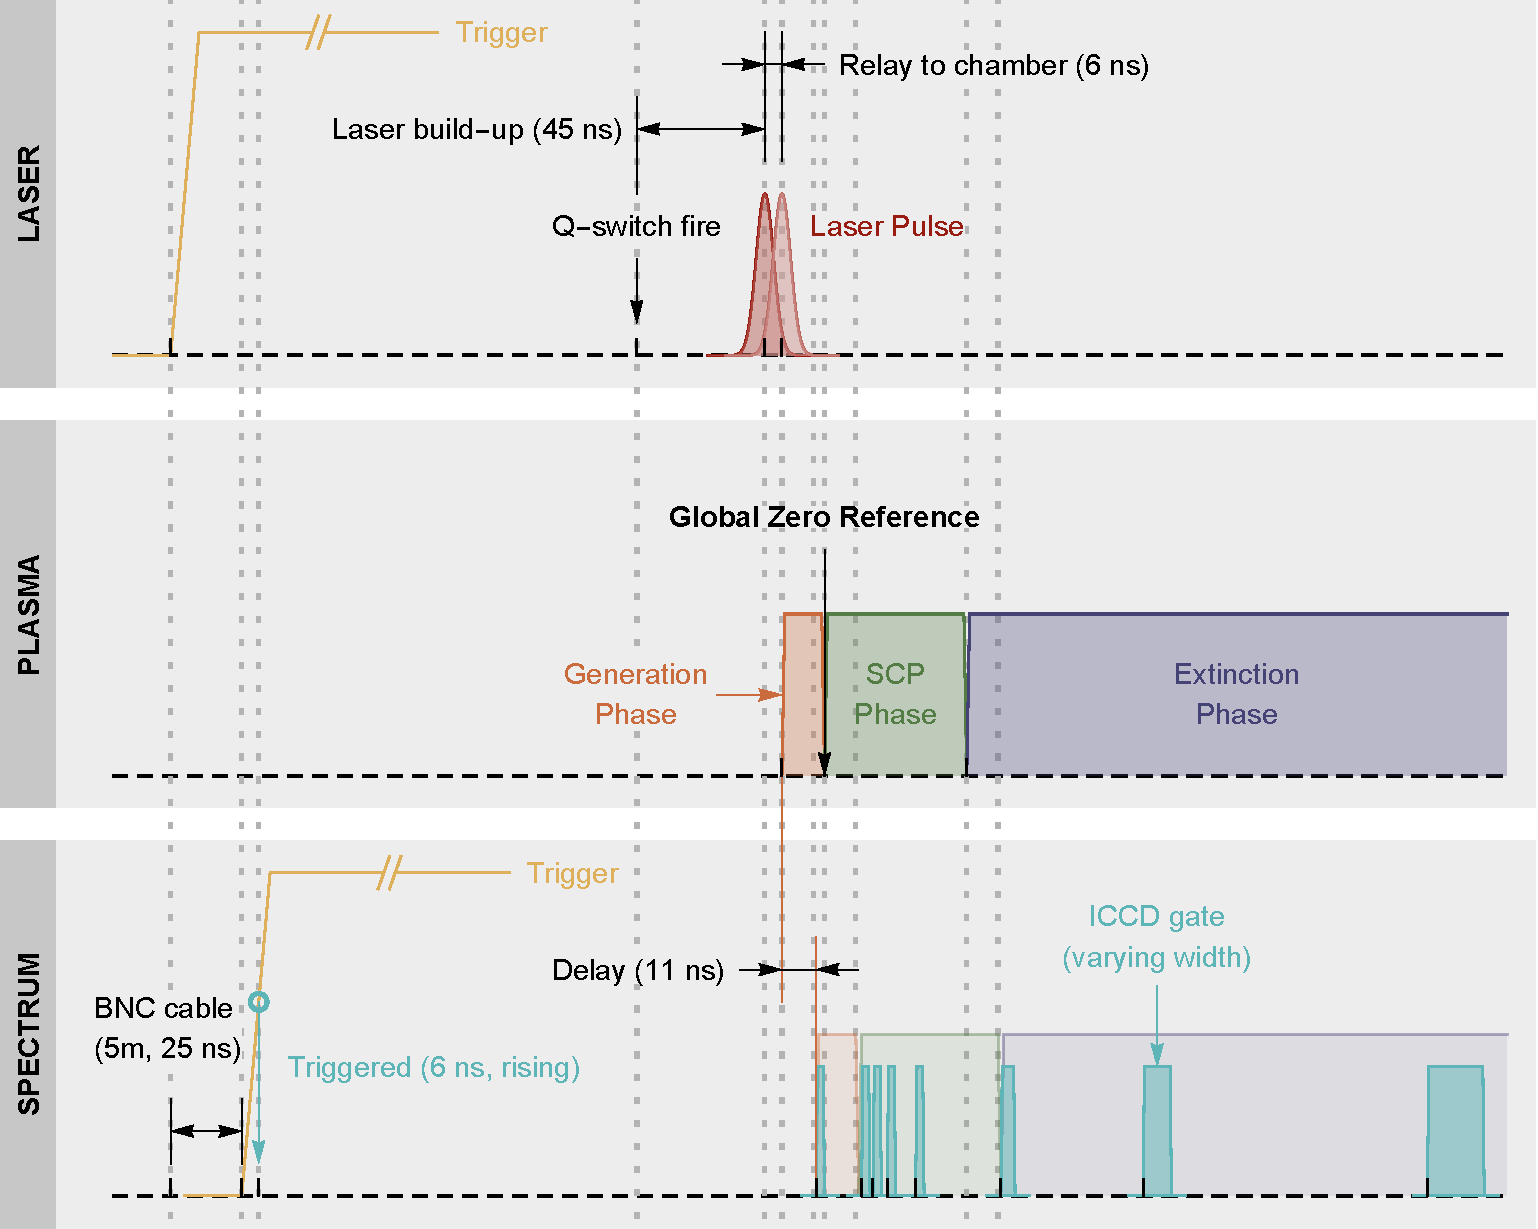
\includegraphics[width=130mm]{figures/ap4/sequence/specSequence.pdf}
\caption{Experimental sequence for measuring emission spectrum from the plasma. The delay time for the emission to reach the detector increases as the relay optics, including the spectrometer, provides a longer optical path length.}
\label{fig:specSequence}
\end{figure}

\begin{figure}[ht!]
\centering
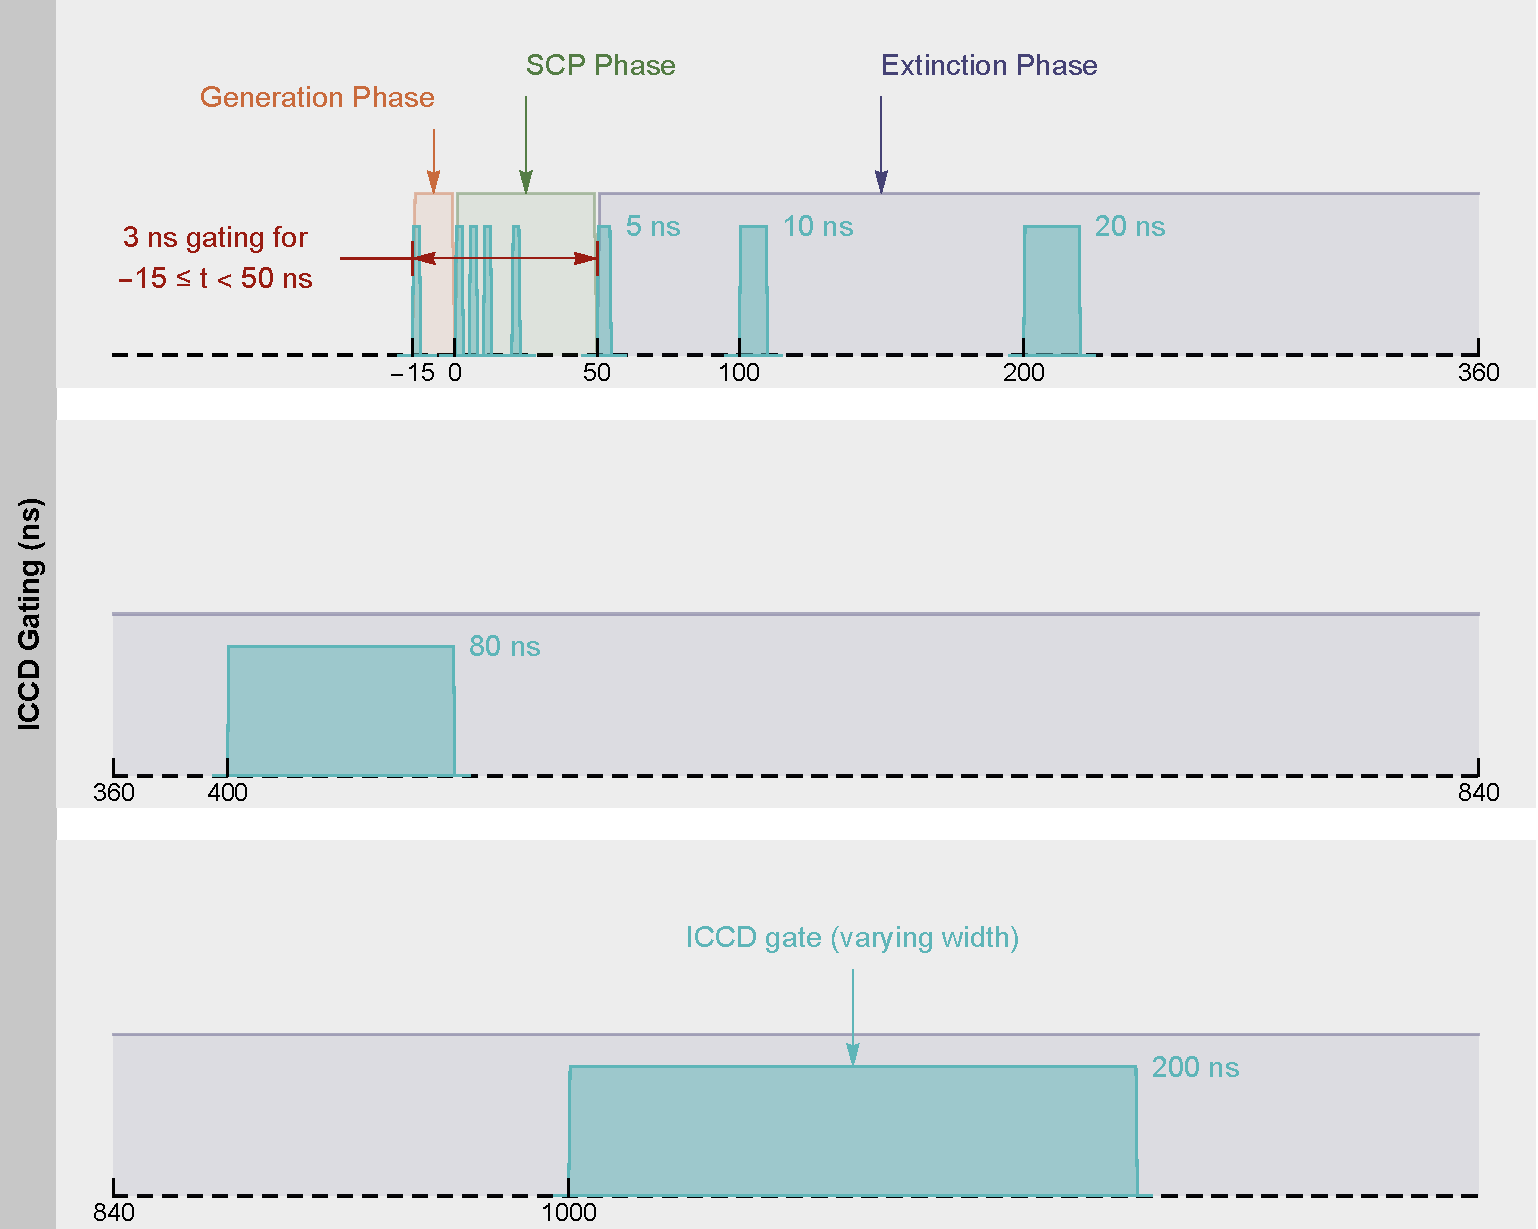
\includegraphics[width=130mm]{figures/ap4/sequence/gatingSequence.pdf}
\caption{Experimental sequence for ICCD gating for both taking images and measuring spectrum.}
\label{fig:gatingSequence}
\end{figure}
